\chapter{Funktionsscharen}

\section{Definition}
\begin{flushleft}
  Eine Funktionsschar ist eine Funktion, die auch von anderen Parametern als \(x\) abhängt.
  \newline
  \[
    f_k(x)=kx^2
  \]
  \newline
  Das ist beispielsweise eine quadratische Funktionsschar, die von den Parametern \(x\) und \(k\) abhängt.
\end{flushleft}

\begin{center}
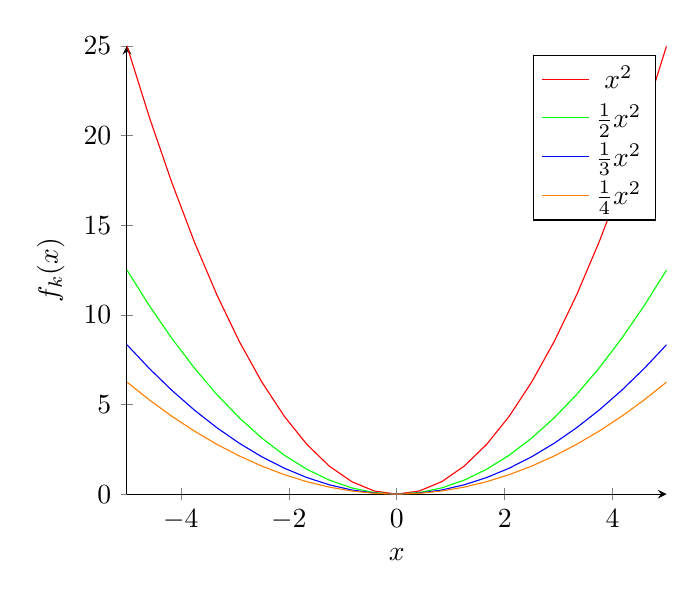
\begin{tikzpicture}
\begin{axis}[
  axis lines = left,
  xlabel = \(x\),
  ylabel = {\(f_k(x)\)}
]
\addplot[
  domain=-5:5,
  samples=25,
  color=red,
]
{x^2};
\addlegendentry{\(x^2\)}

\addplot[
  domain=-5:5,
  samples=25,
  color=green,
]
{0.5*x^2};
\addlegendentry{\(\frac{1}{2}x^2\)}

\addplot[
  domain=-5:5,
  samples=25,
  color=blue,
]
{0.3333*x^2};
\addlegendentry{\(\frac{1}{3}x^2\)}

\addplot[
  domain=-5:5,
  samples=25,
  color=orange,
]
{0.25*x^2};
\addlegendentry{\(\frac{1}{4}x^2\)}

\end{axis}
\end{tikzpicture}
\end{center}

\begin{flushleft}
  Anhand von diesem Beispiel kann man relativ einfach erkennen, dass Funktionen durch Parameter verschiedene Eigenschaften aufweisen können.
\end{flushleft}
